\documentclass[border=2mm]{standalone}
\usepackage{pgfplotstable}
\pgfplotsset{compat=1.14}

\begin{document}

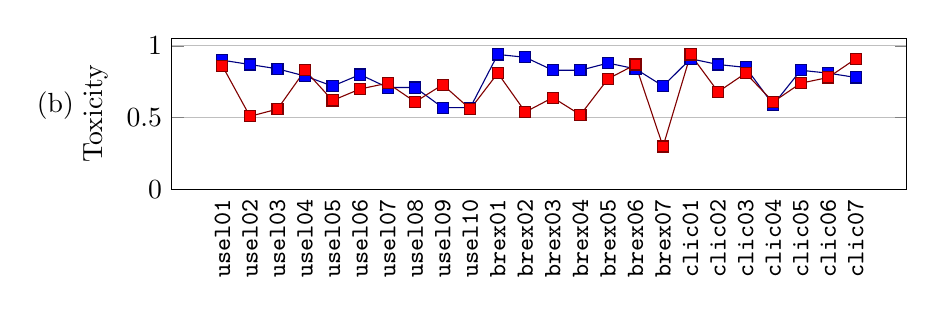
\begin{tikzpicture}
% Configure the axis appearance and layout
\begin{axis}[
    title = (b),
    title style = {at={(-.12,0.45)},anchor=east},
    width  = 0.9*\textwidth,
    height = 3.5cm,
    major x tick style = transparent,
    ymajorgrids = true,
    ymin=0., ymax=1.05,
    ylabel = {Toxicity},
    ylabel near ticks,
    xtick=data,
    symbolic x coords = {usel01,usel02,usel03,usel04,usel05,usel06,usel07,usel08,usel09,usel10, brex01,brex02,brex03,brex04,brex05,brex06,brex07, clic01,clic02,clic03,clic04,clic05,clic06,clic07},
    xticklabel style = {
        rotate=90,            
        font={\ttfamily\small}
    },
    enlarge x limits=0.08
]

% Plot toxicity data for February (first time point)
\addplot+[
    mark=square*,
    mark options={solid, fill=blue},
    color=blue!50!black
] coordinates { 
    (usel01,.90)  (usel02,.87) (usel03,.84) (usel04,.79) (usel05,.72) 
    (usel06,.80)  (usel07,.71) (usel08,.71) (usel09,.57) (usel10,.57) 
    (brex01,.94)  (brex02,.92) (brex03,.83) (brex04,.83) (brex05,.88) 
    (brex06,.84)  (brex07,.72) 
    (clic01,.91)  (clic02,.87) (clic03,.85) (clic04,.59) (clic05,.83) 
    (clic06,.81)  (clic07,.78) 
};

% Plot toxicity data for September (second time point)
\addplot+[
    mark=square*,
    mark options={solid, fill=red},
    color=red!50!black
] coordinates { 
    (usel01,.86)  (usel02,.51) (usel03,.56) (usel04,.83) (usel05,.62) 
    (usel06,.70)  (usel07,.74) (usel08,.61) (usel09,.73) (usel10,.56) 
    (brex01,.81)  (brex02,.54) (brex03,.64) (brex04,.52) (brex05,.77) 
    (brex06,.87)  (brex07,.30) 
    (clic01,.94)  (clic02,.68) (clic03,.81) (clic04,.61) (clic05,.74) 
    (clic06,.78)  (clic07,.91) 
};

\end{axis} 
\end{tikzpicture}

\end{document}
